\documentclass[a4paper]{report}

\usepackage[T1]{fontenc}
\usepackage[utf8]{inputenc}
\usepackage[italian]{babel}
\usepackage{amsmath}
\usepackage{amssymb}
\usepackage{caption}
\usepackage{graphicx}
\usepackage{booktabs}
\usepackage{textcomp}


\begin{document}
\chapter{Supervised Learning e Metodi Statistici}

\section{Introduzione al Supervised Learning}
La scienza delle predizioni, o data learning, gioca un ruolo chiave in diversi campi scientifici come ad esempio quello della statistica e dell'intelligenza artificiale, grazie a procedure applicative legate principalmente al cosiddetto data mining.

In un tipico scenario di apprendimento supervisionato abbiamo un valore di \textit{outcome}, generalmente quantitativo (come ad esempio una quotazione finanziaria) o categorico (come ad esempio una discriminante situazionale del tipo infarto/non infarto), che si vuole predire in base ad un set \textit{features} (ad esempio dati clinici).
Avendo a disposizione un \textit{training set} di dati, dei quali è possibile osservare outcome e features per un insieme di oggetti (ad esempio una popolazione), è dunque opportuno costruire un modello predittivo, o \textit{learner}, il quale permetterà di valutare l'outcome per oggetti ignoti.
\chapter{Valutazione degli effetti di troncatura deterministica per popolazioni sintetiche}

\section{Introduzione al Problema}
L'utilizzo di database spesso composti su un intervallo discreto di una data popolazione, frequentemente selezionato tramite criteri che possiamo definire "deterministici" (un intervallo di età ad esempio, o in generale un certo range di valori disponibile al momento dell'acquisizione), si contrappone all'esigenza di ottenere un modello di validità generale in termini di coefficienti delle variabili e di interazione fra esse.

Non è pertanto possibile elaborare un risultato di questo tipo senza tenere conto di un'analisi quantitativa dell'effetto di slicing dei set di dati, che come è dimostrato in seguito potrà fornire una correzione applicabile al modello sotto forma di stima di un bias per i coefficienti in relazione alla percentuale di dati utilizzati nell'elaborazione.

I risultati di seguito riportati si riferiscono ad interpolazioni di tipo lineare, elaborate attraverso metodi di machine learning quali cross-validation e boot-strapping.

\section{Metodi di Elaborazione}
\subsection {Generazione delle popolazioni e Data Structures}
Le popolazioni sintetiche $x_1$,$x_2$,$x_3$ sono generate in modo da essere distribuite normalmente e la $y$ sia composta secondo la relazione \[y=x_1+0.1x_1^2+x_2x_3\]con l'aggiunta del relativo rumore statistico, anch'esso simulato normalmente.
In questo modo è possibile valutare il bias per termini di primo grado, termini di grado superiore al primo e termini d'interazione (nel caso presente sotto forma di prodotto).

Lo script genera due popolazioni ciascuna composta da $N=10^3$ individui, che successivamente vengono scalate in base alla percentuale di taglio in analisi fornita come argomento alla funzione.

In questo modo sarà sempre possibile confrontare risultati elaborati su popolazioni della stessa grandezza, una composta da elementi selezionati casualmente e che dunque sarà semplicemente una "riduzione in scala" della popolazione iniziale, l'altra composta dagli elementi presenti entro il range percentuale del taglio.

Per quest'ultima categoria di campioni lo slicing viene infatti effettuato dallo script non in maniera stocastica, ma previo sorting del dataset secondo percentili relativi alle posizioni delle singole osservazioni nell'array, vengono eliminati dati a partire dalle estremità in base alla percentuale di slicing fornita come argomento in generazione.

Questa procedura permette di imputare le discrepanze attese relativamente al ranking di modelli ipotetici e stima dei parametri per i coefficienti unicamente al bias dovuto al troncamento deterministico del dataset.

Prima di procedere con la descrizione dei metodi analitici, è utile commentare le strutture utilizzate per manipolare i dati in input; cercando di rendere il programma il più generale possibile è stata infatti introdotta un'organizzazione di tipo Design Matrix, oggetti che descrivono la  composizione matriciale per regressioni multivariate.

Sia un modello di regressione nella forma $y=X\beta+\epsilon$ dove $X$ è la design matrix, $y$ il vettore delle osservazioni sulla variabile dipendente, $\beta$ un vettore di coefficienti associati alle $X_i$ ed $\epsilon $ il vettore dei termini di errore.
Prendendo ad esempio un modello del tipo:
\[y_i = \beta_0 + \beta_1 w_i + \beta_2 x_i + \epsilon_i \]
con 7 osservazioni dipendenti dalle variabili $w$ ed $x$, si ha in termini matriciali:

\[\begin{bmatrix}y_1 \\ y_2 \\ y_3 \\ y_4 \\ y_5 \\ y_6 \\ y_7 \end{bmatrix} =
\begin{bmatrix} 1 & w_1 & x_1  \\1 & w_2 & x_2  \\1 & w_3 & x_3  \\1 & w_4 & x_4  \\1 & w_5 & x_5  \\1 & w_6 & x_6 \\ 1& w_7  & x_7  \end{bmatrix}
\begin{bmatrix} \beta_0 \\ \beta_1 \\ \beta_2  \end{bmatrix}
+
\begin{bmatrix} \epsilon_1 \\ \epsilon_2 \\ \epsilon_3 \\ \epsilon_4 \\ \epsilon_5 \\ \epsilon_6 \\ \epsilon_7 \end{bmatrix}\]
Convenzionalmente, ed anche all'interno del programma utilizzato, la matrice delle $y$ è definita come "Outcome" e quella delle $X$ come "Predictor"; in questo modo è possibile generalizzare l'elaborazione senza dover definire funzioni specifiche in relazione al numero ed al tipo di variabili introdotte.

L'analisi è dunque strutturata in due parti specifiche per valutare l'effetto di slicing su quelli che sono aspetti essenziali per l'attribuzione della capacità predittiva di un dato metodo: il ranking di modelli ipotetici per $y$, ovviamente noto quello utilizzato per la generazione, e la precisione nella stima dei coefficienti per  le $x$.

\subsection{Effetto della troncatura nell'attribuzione dello score per modelli ipotetici}
L'algoritmo utilizzato per questo tipo di analisi prevede l'uso di tecniche di Cross Validation (nel caso specifico K-Fold Cross Validation) per il calcolo della bontà di previsione del regressore fornito,  una semplice interpolazione lineare multivariata, con il quale lo script procede ad elaborare un array contenente dei modelli ipotetici, incluso quello utilizzato per la generazione delle $y$ e che può dunque essere preso come riferimento, valutandone un $R^2$ "generalizzato" tramite una popolazione di validazione selezionata casualmente a cui vengono applicati i vari coefficienti calcolati su stratificazioni di popolazioni di Train e Test diverse per ogni iterazione, anch'esse ottenute tramite random shuffling.

In questo modo è possibile simulare l'effetto di perdita di dati sensibili a causa di criteri di selezione dei campioni o in generale l'utilizzo di un range discreto di occorrenze.

L'array dei modelli di prova contiene ipotesi riferite ai singoli termini, a tutte le loro possibili combinazioni lineari, alle possibili interazioni a coppie ed a strutture più vicine al modello di generazione e dunque contenenti termini di grado superiore al primo.
Di seguito sono riportate alcune tabelle di ranking riferite a diverse percentuali di troncatura.

\begin{table}[h!btp]
\begin{tabular}{lrrrr}
\toprule
{} &  entire &  sliced &  entire val. &  sliced val. \\
\midrule
y$\sim$x2*x3+I(x1**2)+x1 &         0.685 &         0.684 &             0.665 &             0.664 \\
y$\sim$x2*x3+x1          &         0.678 &         0.678 &             0.665 &             0.664 \\
y$\sim$x2*x3             &         0.353 &         0.347 &             0.319 &             0.319 \\
y$\sim$x2*x3+I(x1**2)    &         0.345 &         0.345 &             0.331 &             0.332 \\
y$\sim$x1 + x2           &         0.315 &         0.314 &             0.314 &             0.318 \\
y $\sim$ x1              &         0.311 &         0.312 &             0.323 &             0.322 \\
y $\sim$ x1 * x2         &         0.312 &         0.312 &             0.319 &             0.323 \\
y$\sim$x1+x2+x3          &         0.313 &         0.312 &             0.323 &             0.328 \\
y$\sim$x1+x3             &         0.310 &         0.310 &             0.314 &             0.311 \\
y$\sim$x1*x3             &         0.307 &         0.307 &             0.327 &             0.325 \\
y$\sim$x3                &        -0.009 &        -0.011 &            -0.001 &            -0.002 \\
y $\sim$ x2              &        -0.005 &        -0.011 &            -0.005 &            -0.002 \\
\bottomrule
\end{tabular}
\caption{\textit{La tabella contiene gli scores relativi alle prove per popolazioni intere e tagliate ed i corrispondenti punteggi  ottenuti su popolazioni di validazione, in questo caso la percentuale di utilizzo del database è massima.}}
\end{table}

\begin{table}[h!btp]
\begin{tabular}{lrrrr}
\toprule
{} &  entire &  sliced &  entire val. &  sliced val. \\
\midrule
y$\sim$x2*x3+I(x1**2)+x1 &         0.659 &         0.260 &             0.665 &             0.494 \\
y$\sim$x2*x3+x1          &         0.646 &         0.256 &             0.664 &             0.482 \\
y $\sim$ x1              &         0.308 &         0.134 &             0.326 &             0.209 \\
y$\sim$x1 + x2           &         0.309 &         0.131 &             0.339 &             0.213 \\
y$\sim$x1+x3             &         0.306 &         0.130 &             0.329 &             0.209 \\
y$\sim$x1*x3             &         0.299 &         0.130 &             0.335 &             0.211 \\
y $\sim$ x1 * x2         &         0.303 &         0.128 &             0.330 &             0.211 \\
y$\sim$x1+x2+x3          &         0.306 &         0.128 &             0.323 &             0.210 \\
y$\sim$x2*x3             &         0.354 &         0.048 &             0.306 &             0.186 \\
y$\sim$x2*x3+I(x1**2)    &         0.352 &         0.042 &             0.338 &             0.192 \\
y $\sim$ x2              &        -0.019 &        -0.013 &            -0.005 &            -0.003 \\
y$\sim$x3                &        -0.023 &        -0.015 &            -0.001 &            -0.001 \\
\bottomrule
\end{tabular}
\caption{\textit{La tabella contiene gli scores relativi alle prove per popolazioni intere e tagliate ed i corrispondenti punteggi  ottenuti su popolazioni di validazione, in questo caso la percentuale di utilizzo del database è del 66\%.}}
\end{table}

\begin{table}[h!btp]
\begin{tabular}{lrrrr}
\toprule
{} &  entire &  sliced &  entire val. &  sliced val. \\
\midrule
y$\sim$x2*x3+x1          &         0.495 &         0.011 &             0.658 &             0.148 \\
y$\sim$x2*x3+I(x1**2)+x1 &         0.510 &         0.005 &             0.660 &             0.146 \\
y$\sim$x1+x3             &         0.215 &        -0.031 &             0.285 &             0.049 \\
y $\sim$ x1              &         0.218 &        -0.041 &             0.319 &             0.050 \\
y$\sim$x1*x3             &         0.215 &        -0.045 &             0.330 &             0.049 \\
y$\sim$x1+x2+x3          &         0.227 &        -0.047 &             0.269 &             0.046 \\
y$\sim$x2*x3             &         0.117 &        -0.058 &             0.319 &             0.047 \\
y$\sim$x3                &        -0.131 &        -0.058 &            -0.009 &            -0.001 \\
y$\sim$x1 + x2           &         0.231 &        -0.059 &             0.310 &             0.049 \\
y $\sim$ x1 * x2         &         0.225 &        -0.070 &             0.269 &             0.046 \\
y$\sim$x2*x3+I(x1**2)    &         0.094 &        -0.076 &             0.346 &             0.047 \\
y $\sim$ x2              &        -0.094 &        -0.091 &            -0.038 &            -0.005 \\
\bottomrule
\end{tabular}
\caption{\textit{La tabella contiene gli scores relativi alle prove per popolazioni intere e tagliate ed i corrispondenti punteggi  ottenuti su popolazioni di validazione, in questo caso la percentuale di utilizzo del database è del 33\%}.}
\end{table}
Come si vede dai risultati, la classifica dei modelli in relazione alla stima del peso dei termini è in generale mantenuta anche per perdite considerevoli di dati mentre la qualità della previsione riferita alle popolazioni tagliate peggiora notevolmente; resta quindi da determinare l'andamento della stima dei coefficienti in relazione alla percentuale di utilizzo dei datasets.

\subsection{Effetto della troncatura nella stima dei coefficienti }

Per la stima del bias sui coefficienti è stato necessario valutare il rapporto fra coefficienti calcolati su popolazioni intere e coefficienti ottenuti da quelle  tagliate in corrispondenza all'aumento della percentuale di dati rimossi.

 Le funzioni utilizzate per questa sezione dell'analisi sono le stesse della precedente, con l'aggiunta di un metodo che permette di accedere ai parametri per i singoli termini del modello e di un ciclo di elaborazione statstica che consente  di utilizzare mediane e deviazioni standard per il plotting.
I grafici seguenti mostrano l'andamento dei rapporti per steps di slicing del 10\%.

\begin{figure}[hbtp]
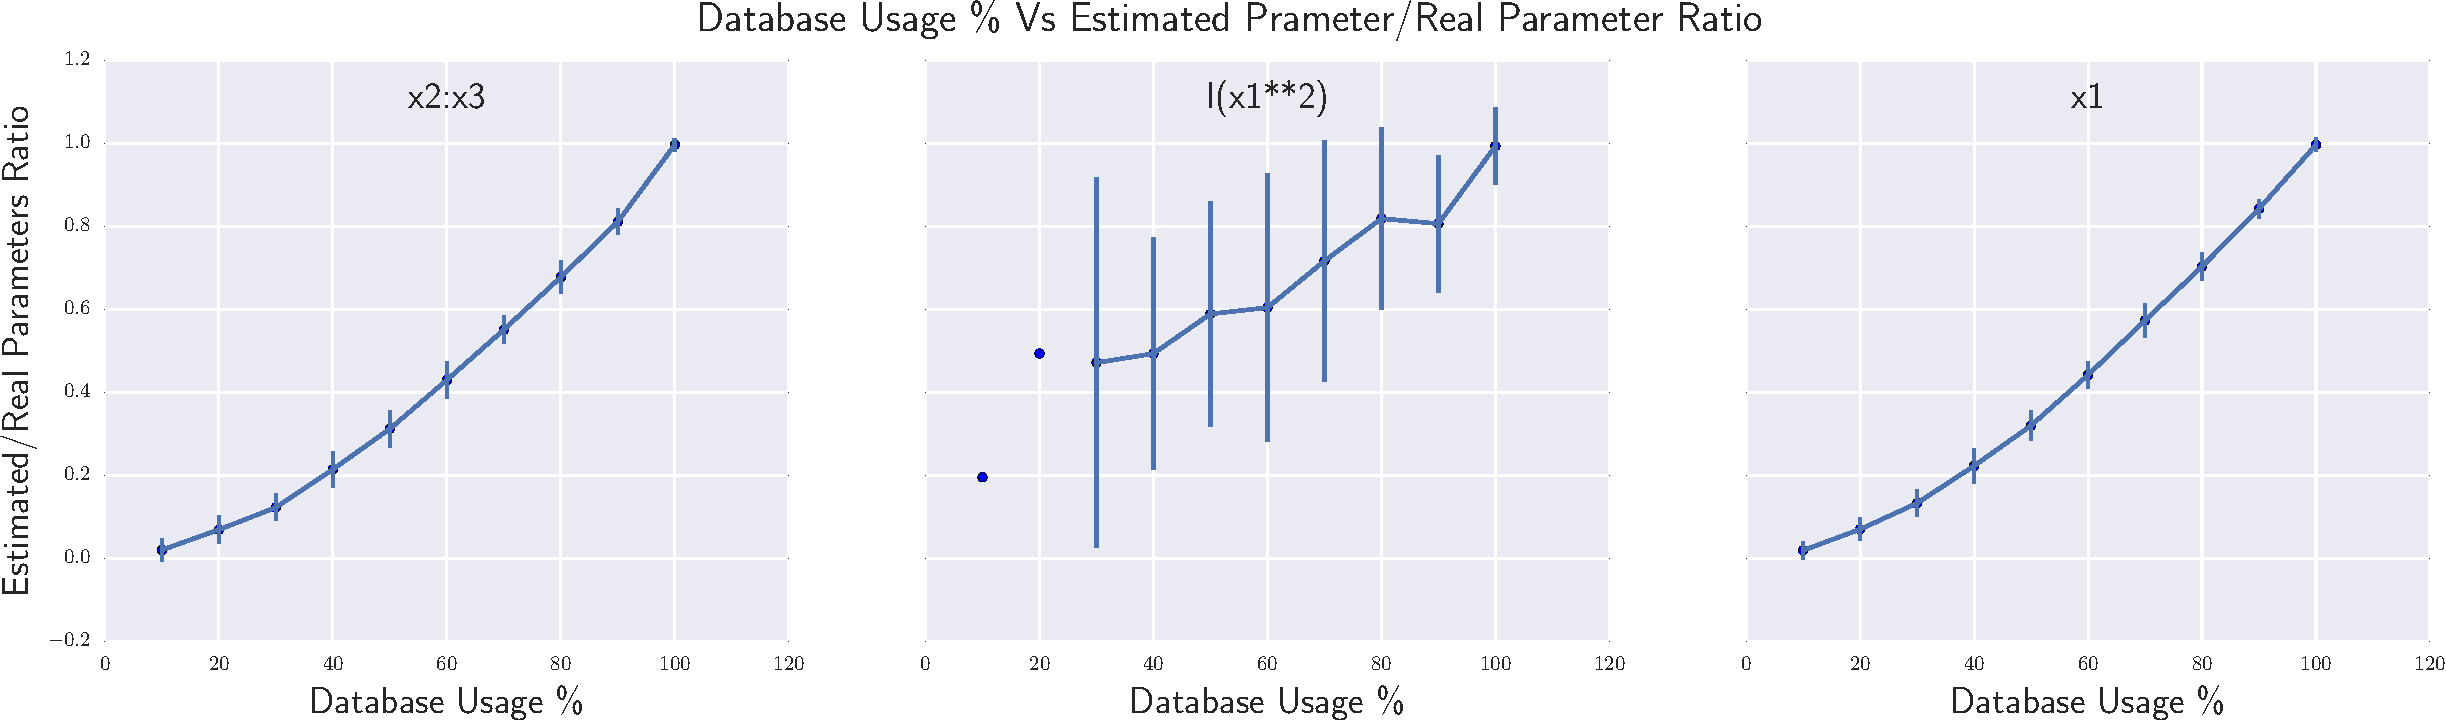
\includegraphics[width=\textwidth]{finalgraph}
\caption{\textit{Plotting della variazione del rapporto fra coefficienti in relazione al taglio del dataset. Come è evidente dal grafico al centro l'errore aumenta considerevolmente per il parametro associato al termine di grado superiore al primo a causa della sua vicinanza allo zero.}}
\end{figure}


Si può notare come l'effetto della troncatura abbia nelle migliori delle ipotesi, ossia per un'analisi fatta con dati sintetici distribuiti normalmente, un andamento lievemente esponenziale e dunque tutt'altro che trascurabile.

\end{document}